\section{Auswertung}
\label{sec:auswertung}
In diesem kapitel sollen die gemessenen Werte ausgewertet werden und zueineander in Verbindung gebracht werden.
\subsection{Emissionspektrum der Kupferröntgenröhre}
\label{sec:emskupfer}
Zunächst wurden die gemessenen Werte, wie in \autoref{fig:kupfer} zu sehen, geplottet.
Auf der linken Seite der Grafik ist zunächst ein leichter Bremsberg zu erkenne dann folgt der kleinere
$K_{\beta}$- und der größere $K_{\alpha}$-Peak. Ihre rechte Flanke ist jeweils die Absorbtionslinie.
Um die Energie dieser Linie zu erhalten, wurden die in rot markierten Maxima und Minima gesucht und
durch das jeweilige Punktepaar eine Gerade gelegt deren Mitte über 
$N_{Mitte}=N_{min}+\frac{N_{max}-N_{min}}{2}$ bestimmt wurde. Aus den so erhaltenen Winkeln kann sofort über
\begin{center}
    $E=\frac{hc}{2d_{LiF}sin(\Theta)}$
\end{center}
die Energie der Linien bestimmt werden. Sie liegen mit folgenden Winkeln $\Theta$ bei:
\begin{center}
    $\Theta_{\alpha}=\SI[]{23.70}[]{°}$\\
    $\Theta_{\beta}=\SI[]{20.95}[]{°}$\\
\end{center}
\begin{center}
    $E_{\alpha}=\SI[]{1.3792\times 10^{-27}}[]{J}$\\
    $E_{\beta}=\SI[]{1.2269\times 10^{-27}}[]{J}$\\
\end{center}
\begin{figure}
    \centering
    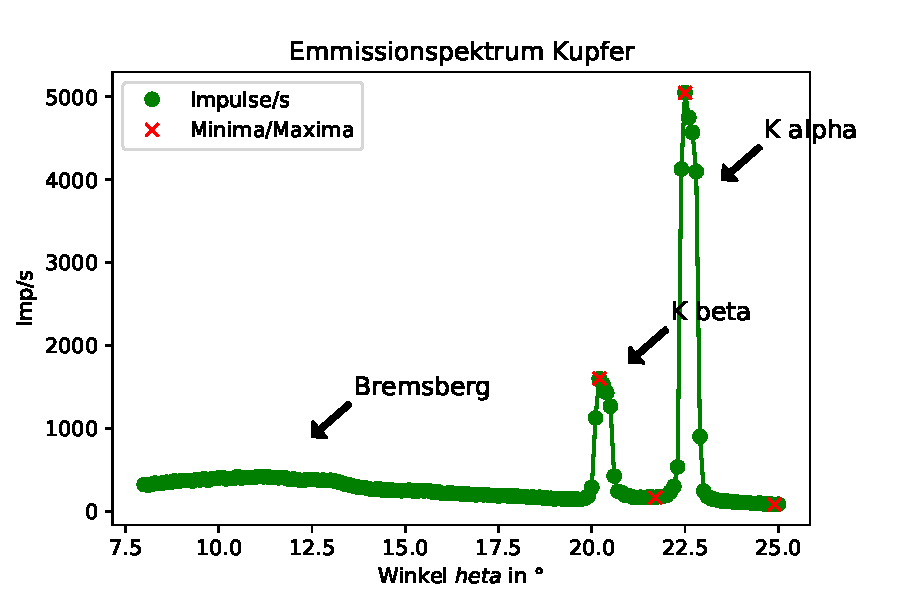
\includegraphics{Kupfer.pdf}
    \caption{Emissionspektrum der Kupfer Kathode}
    \label{fig:kupfer}
  \end{figure}

\subsection{Bestimmung der Transmission als Funktion der Wellenlänge}
\label{sec:transmission}
Zur bestimmung der wellenlängenabängigien Transmission wurde der Winkelbreich $7°$-$10°$ doppelt vermessen,
zunächst ohne Aluminium-Absorber dann nocheinmal mit. Die gemessenen Daten wurden dann über $\lambda=2d_{lif}sin(\Theta)$
in Wellenlängen umgerechnet und mit $I=\frac{N}{1-\tau N}$ die Totzeit $\tau=\SI[]{90}[]{\mu s}$ des 
Geiger-Müller-Zählrohres korrigiert. Mit $T=\frac{I_{Al}}{I_0}$ konnte dann sofort die Transmission bestimmt
werden. Zudem wurde noch eine lineare Ausgleichsgrade, der Form $T=mx+b$ mit den koeffizienten:
\begin{center}
    $a=-0.015 \pm 0.0$\\
    $b=1.225 \pm 0.014$
\end{center}
durch die Daten gelgegt. Das Ergebnis ist in \autoref{fig:spektrum} zu sehen.

\begin{figure}
    \centering
    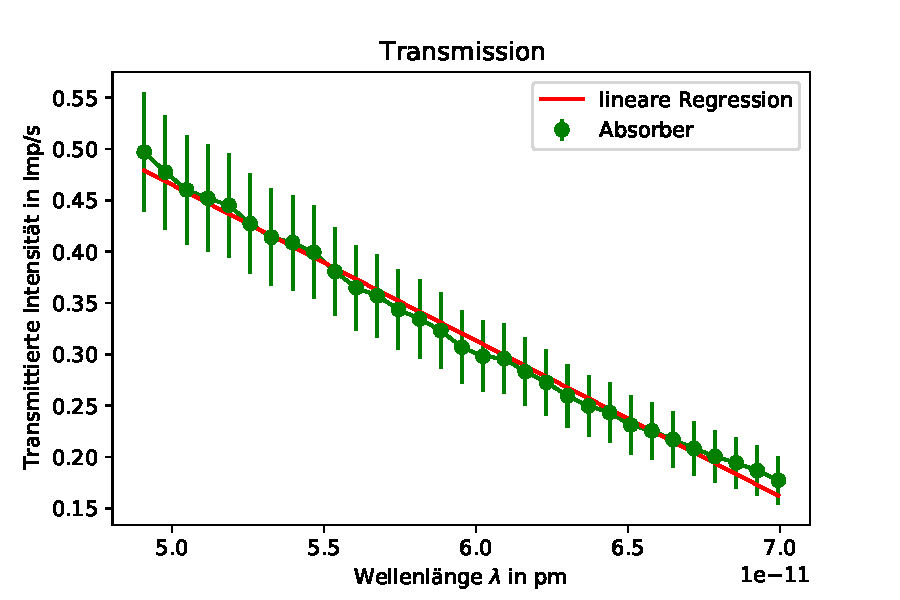
\includegraphics{spektrum.pdf}
    \caption{Transmission als Funktion der Wellenlänge}
    \label{fig:spektrum}
  \end{figure}

\subsection{Bestimmung der Compton Wellenlänge}
\label{sec:compton}
Um die Comptonwellenlänge zu erhalten wurde zweifach gemessen, einmal mit einem 
Aluminium-Absorber zwischen Röntgenquelle und Streukörper und einmal mit dem Absorber zwischen Streukörper
und Geiger-Müller-Zählrohr. Die erhaltenen Werte:
\begin{center}
    $I_0=\SI[]{2731}[]{Imp}$\\
    $I_1=\SI[]{1180}[]{Imp}$\\
    $I_2=\SI[]{1024}[]{Imp}$\\
\end{center}
wurden über $T_1=\frac{I_1}{I_0}=0.4321$ und $T_2=\frac{I_2}{I_0}=0.3750$ verrechnet. Diese Werte liegen auf der
in \autoref{sec:transmission} berechneten Ausgleichsgrade bei Wellenflängen von $\lambda_1=\SI[]{52.1889}[]{pm}$
und $\lambda_2=\SI[]{55.9482}[]{pm}$. Das ergibt mit $\lambda_c=\lambda_2 -\lambda_1$ eine Comptonwelllenlänge
von $\lambda_c=\SI[]{3.7593}[]{pm}$. Eine Totzeitkorrektur ist bei sehr kleinen Zählraten nicht erforderlich da 
es sehr unwahrscheinlich ist das ein Impuls in der Totzeit liegt wenn die Totzeit $\tau$ sehr viel kleiner ist
als das mittlere Intervall zwischen zwei Impulsen.